\subsection*{Simple Model}

        The simplest possible model is the one in which the number of nucleotides determines the read duration,
        possibly with some constant term for getting started.  To consider this, we start with a scatterplot of
        bases against time with a linear fit.

        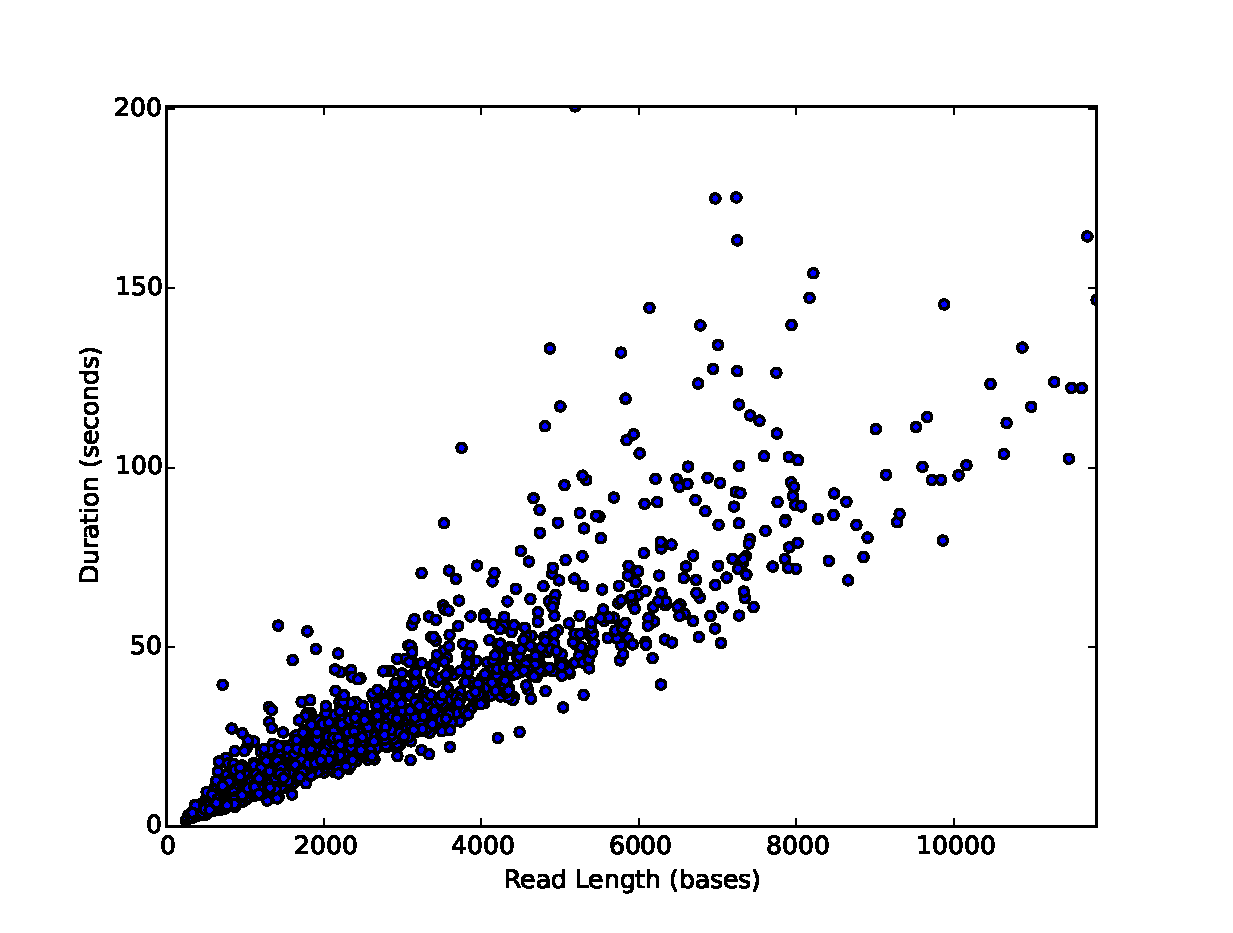
\includegraphics[width=3in]{part11scatterbd}

        We might be tempted to include a constant term in our fitting, but as should be apparent, it would be
        negative.  How long it would take to sequence an extremely short read is unclear.  Fortunately, there 
        are none in our sample.
        
Cost per nucleotide: 11.25ms\\
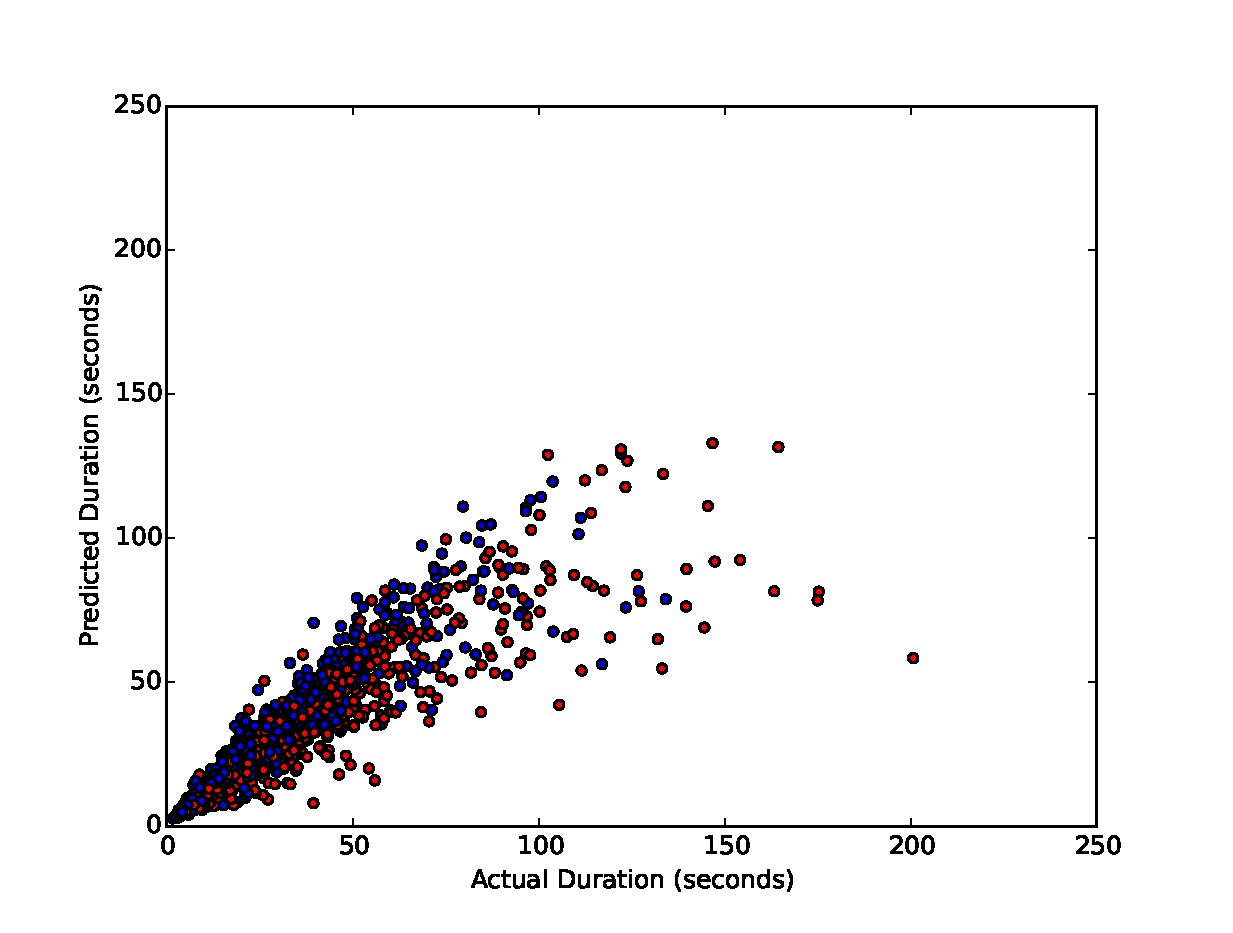
\includegraphics[width=4in]{part11scatter0mer}

$r^2=0.84$


(Red circles are template strand; blue are complement.  There appears to be no significant difference between them.)

\subsection*{Nucleotide Model}
Cost per nucleotide: 
A=32ms 
C=-07ms 
G=04ms 
T=12ms 


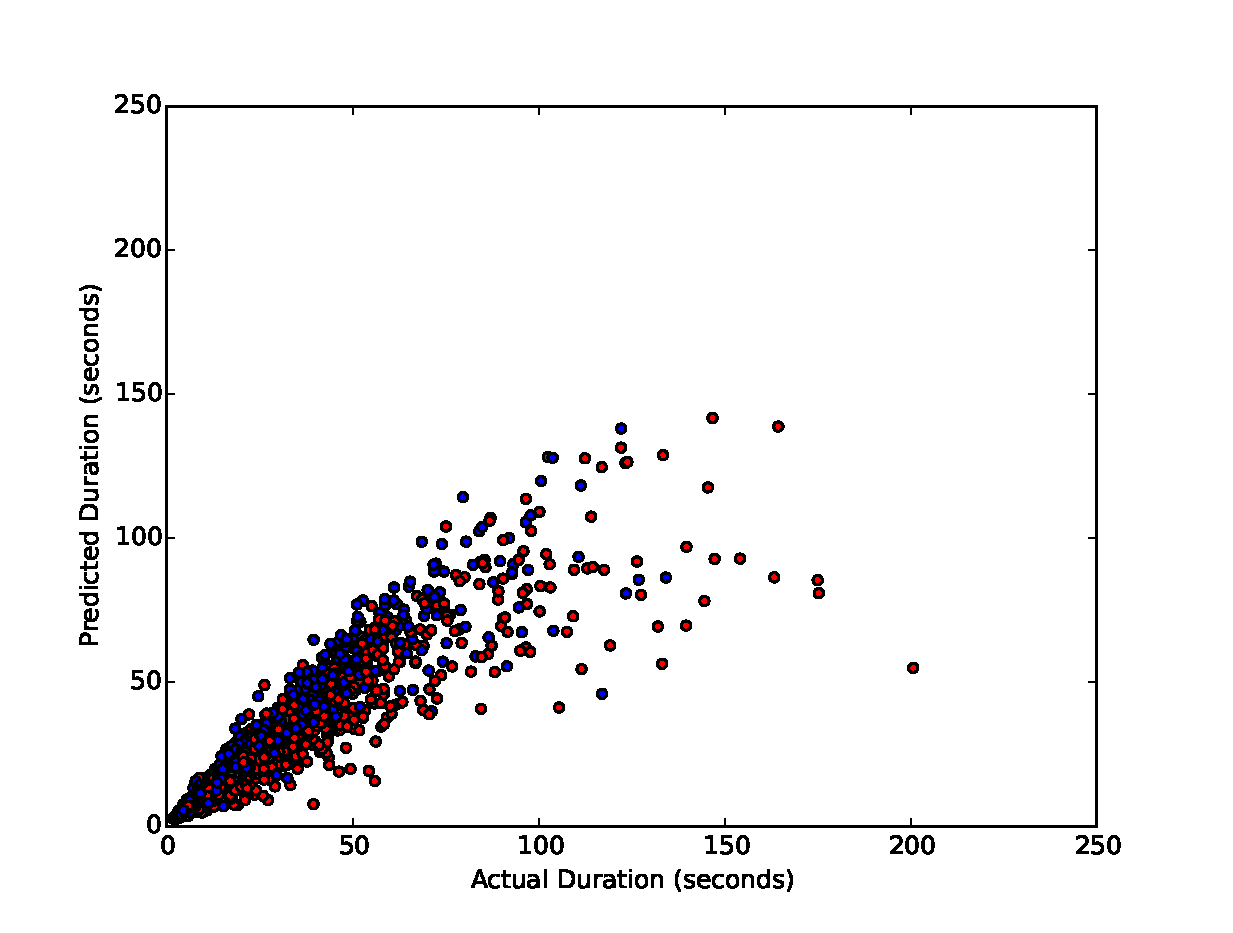
\includegraphics[width=4in]{part11scatter1mer}

$r^2=0.84$

\subsection*{2mer Model}

        We can use a model in which each the time to extend by one nucleotide is determined by the 2-mer in the middle of the
        pore.  We can not list all the costs, but here's a histogram:
        
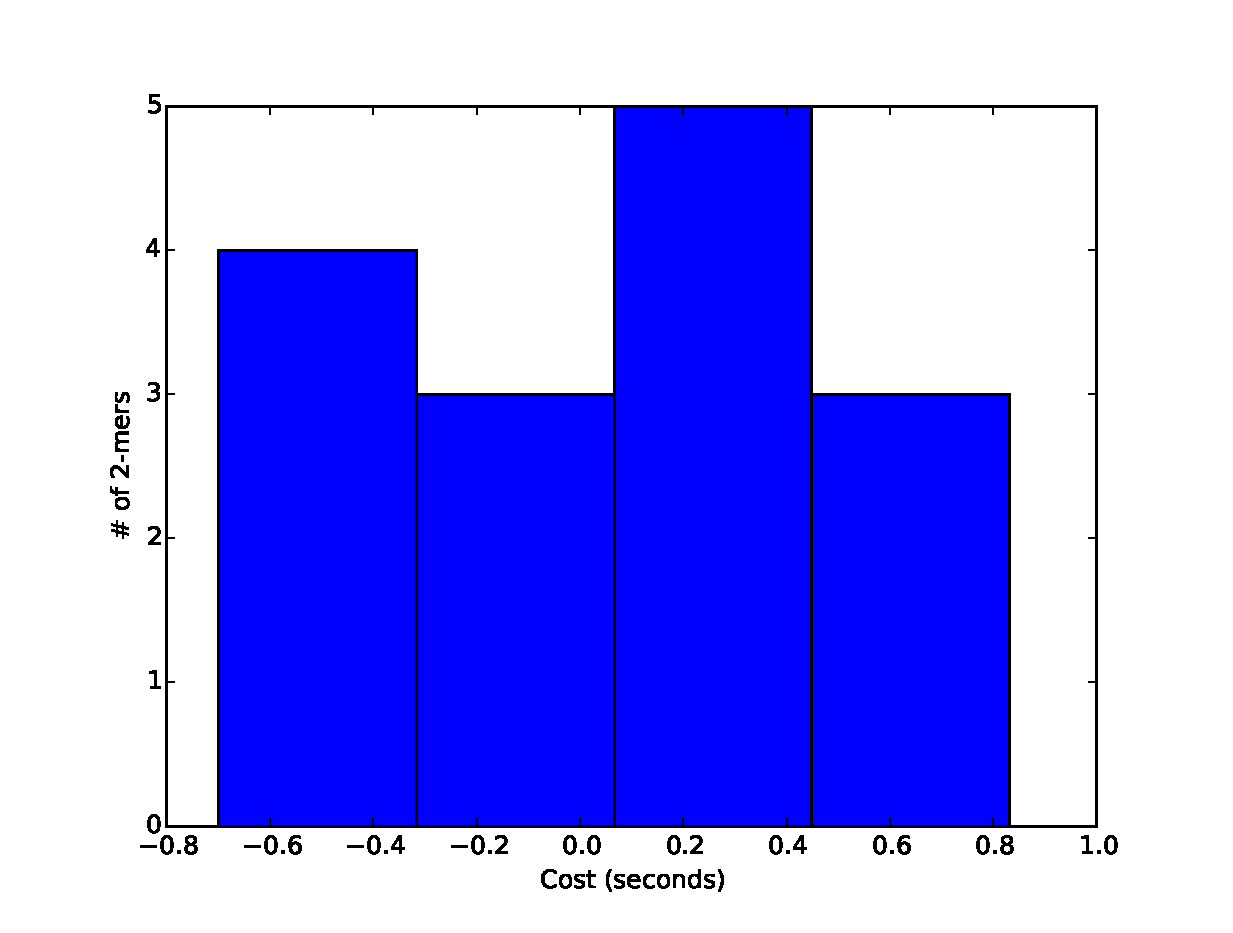
\includegraphics[width=3in]{part11hist2}\\
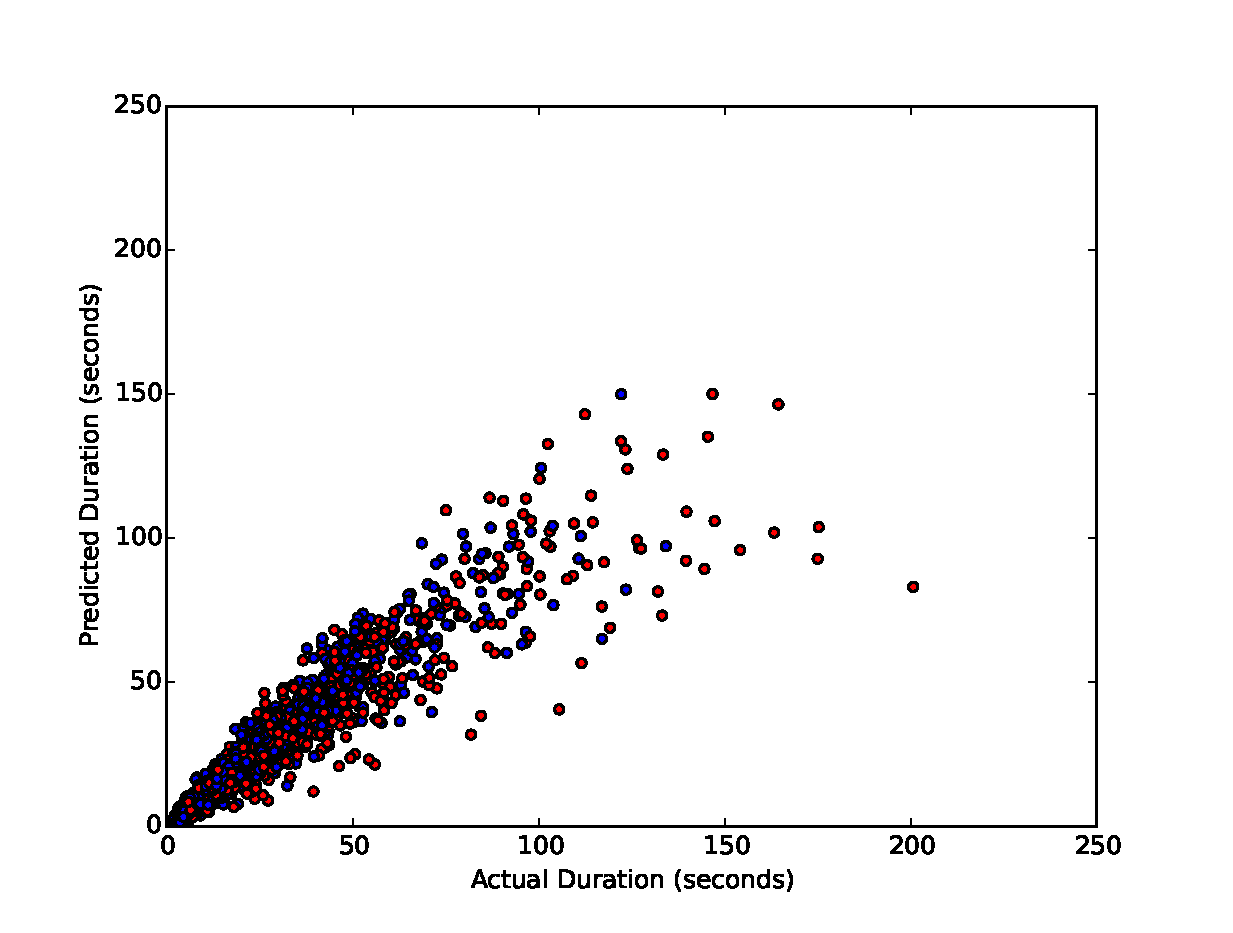
\includegraphics[width=4in]{part11scatter2mer}

$r^2=0.88$

\subsection*{3mer Model}

        We can use a model in which each the time to extend by one nucleotide is determined by the 3-mer in the middle of the
        pore.  We can not list all the costs, but here's a histogram:
        
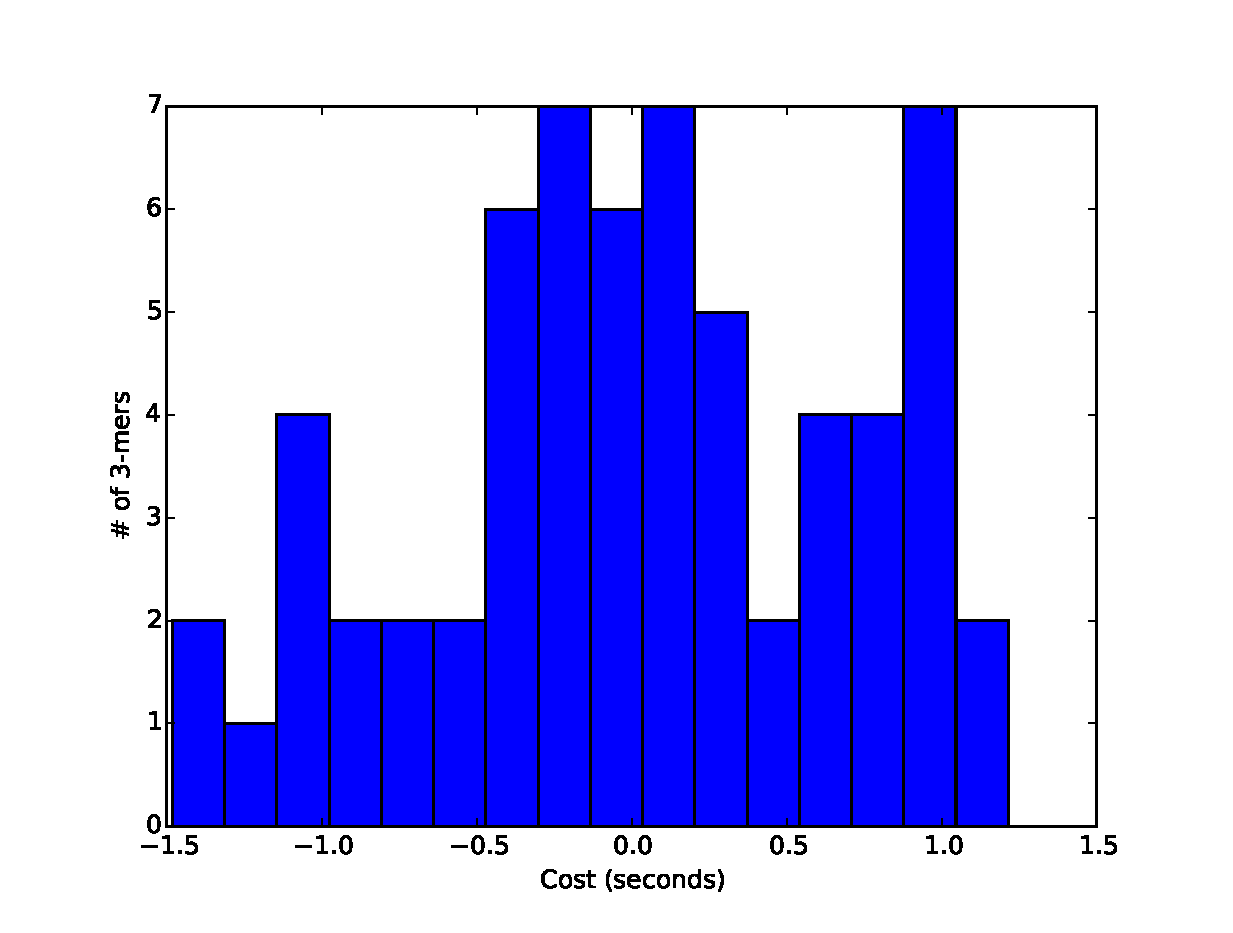
\includegraphics[width=3in]{part11hist3}\\
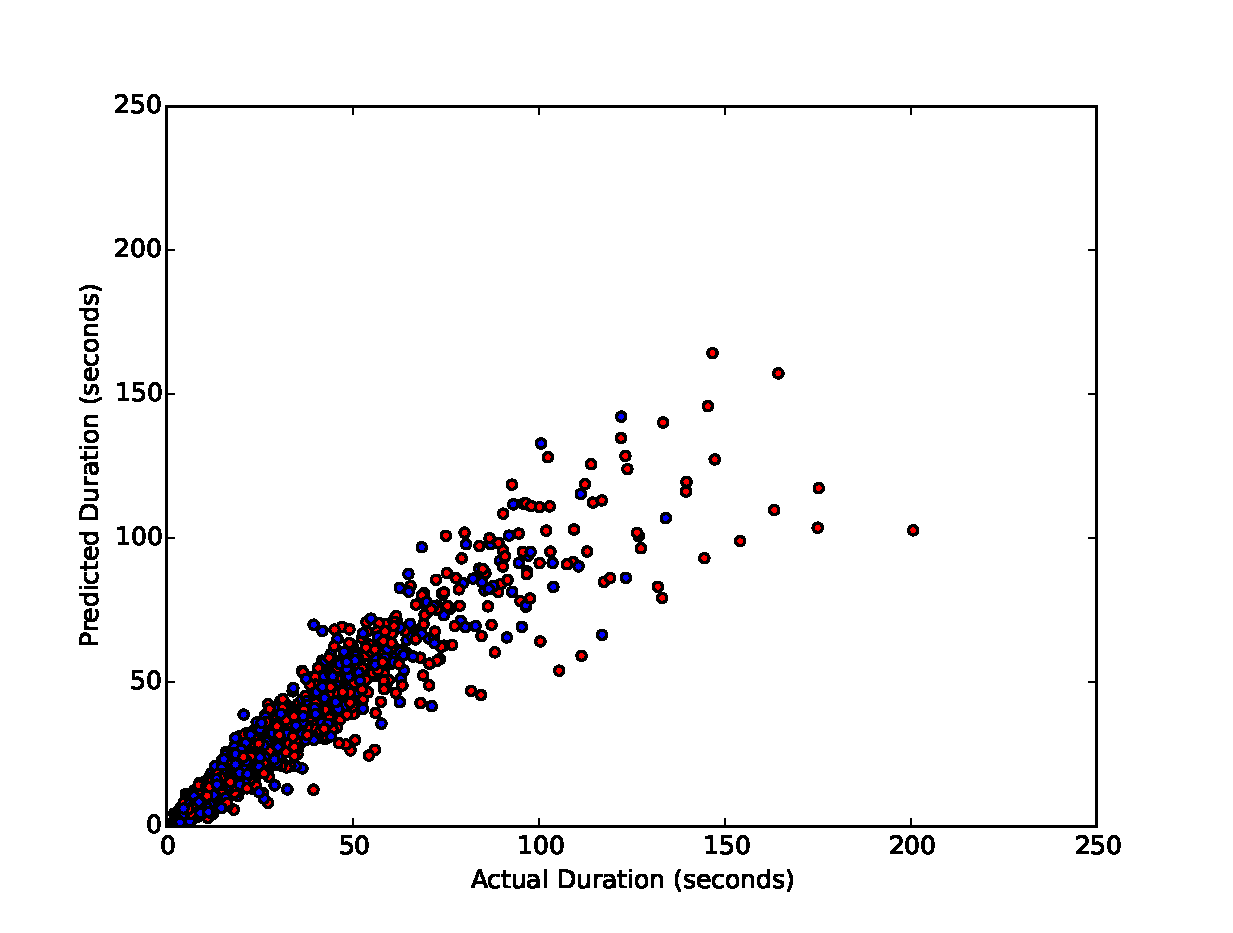
\includegraphics[width=4in]{part11scatter3mer}

$r^2=0.91$

\subsection*{4mer Model}

        We can use a model in which each the time to extend by one nucleotide is determined by the 4-mer in the middle of the
        pore.  We can not list all the costs, but here's a histogram:
        
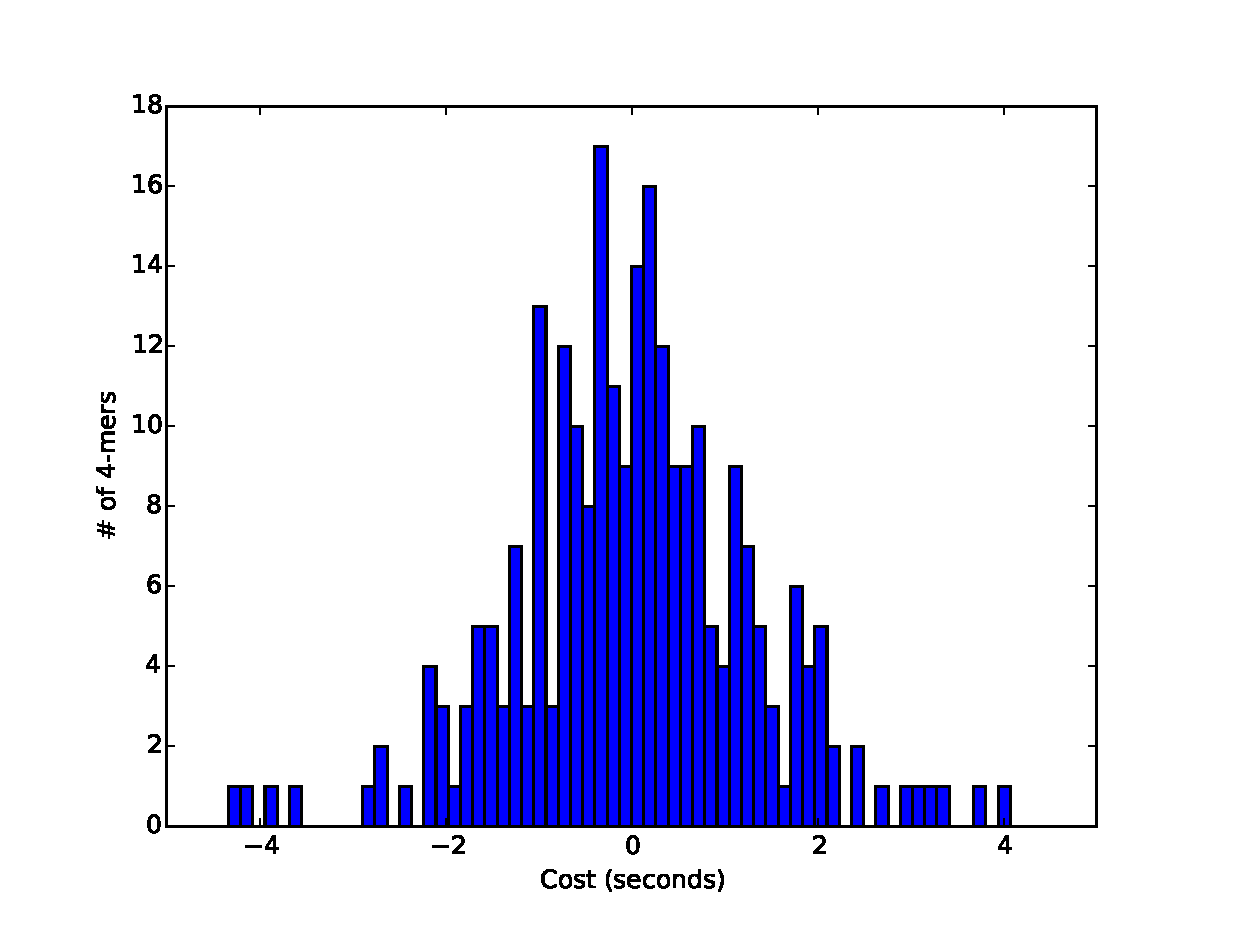
\includegraphics[width=3in]{part11hist4}\\
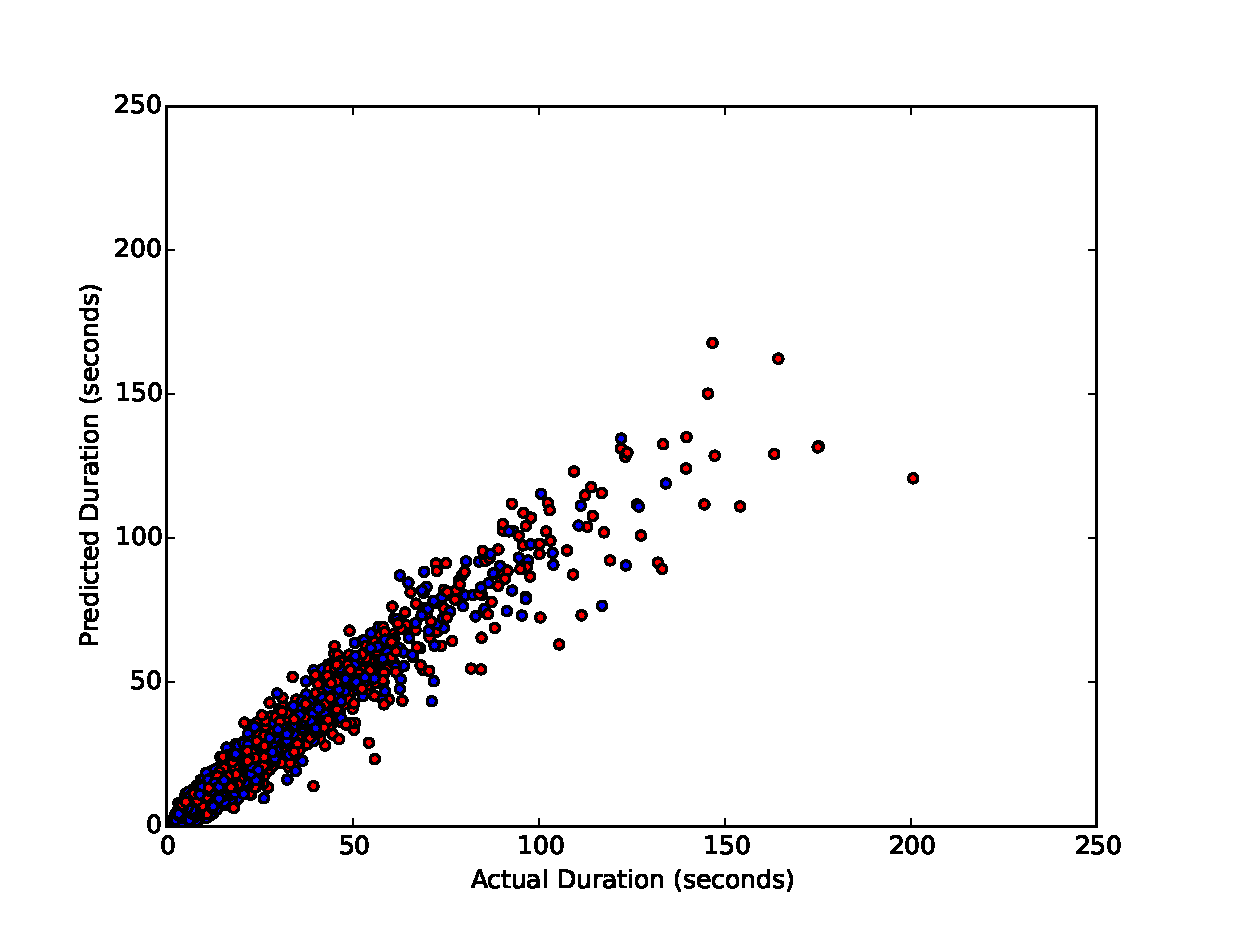
\includegraphics[width=4in]{part11scatter4mer}

$r^2=0.94$

\subsection*{5mer Model}

        We can use a model in which each the time to extend by one nucleotide is determined by the 5-mer in the middle of the
        pore.  We can not list all the costs, but here's a histogram:
        
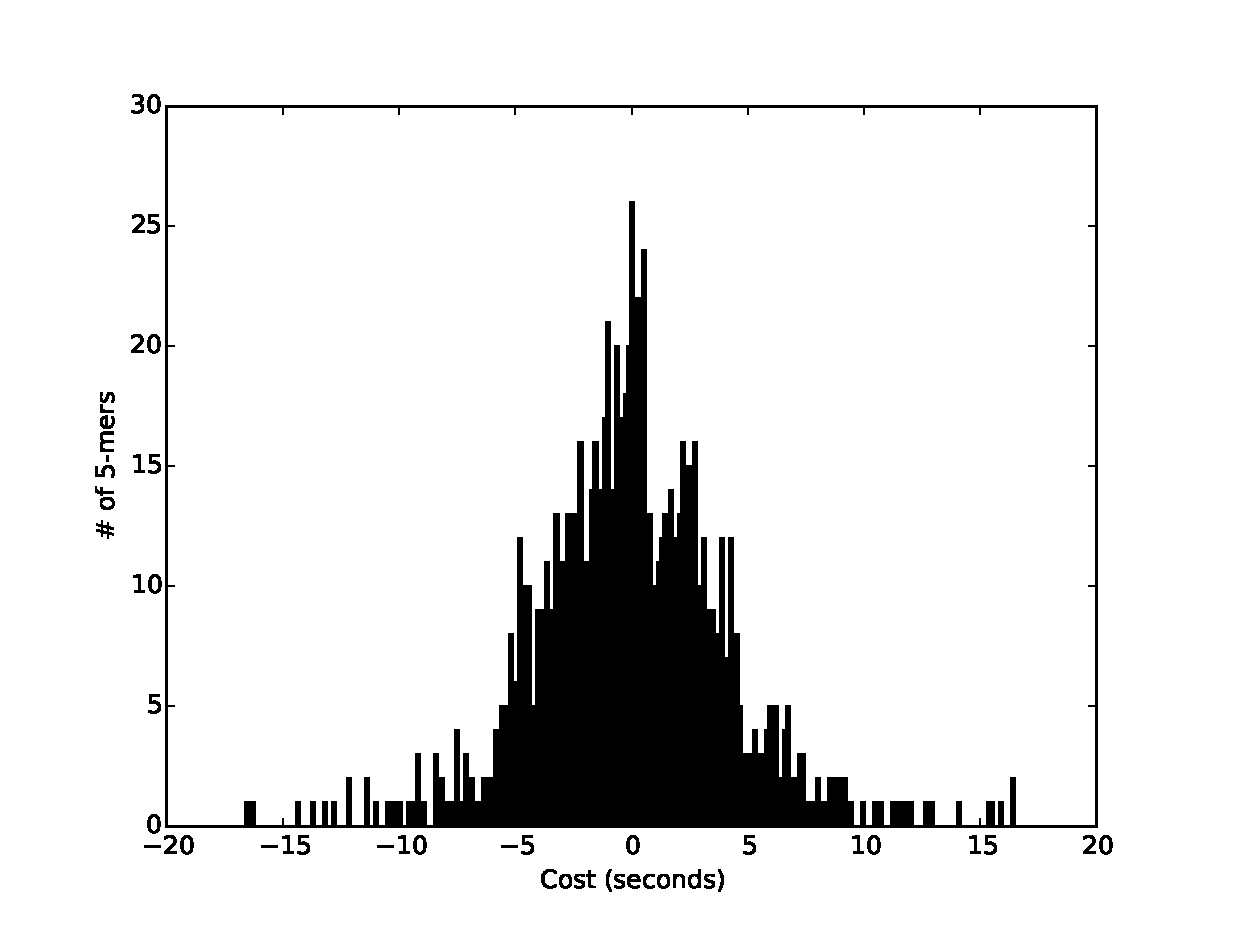
\includegraphics[width=3in]{part11hist5}\\
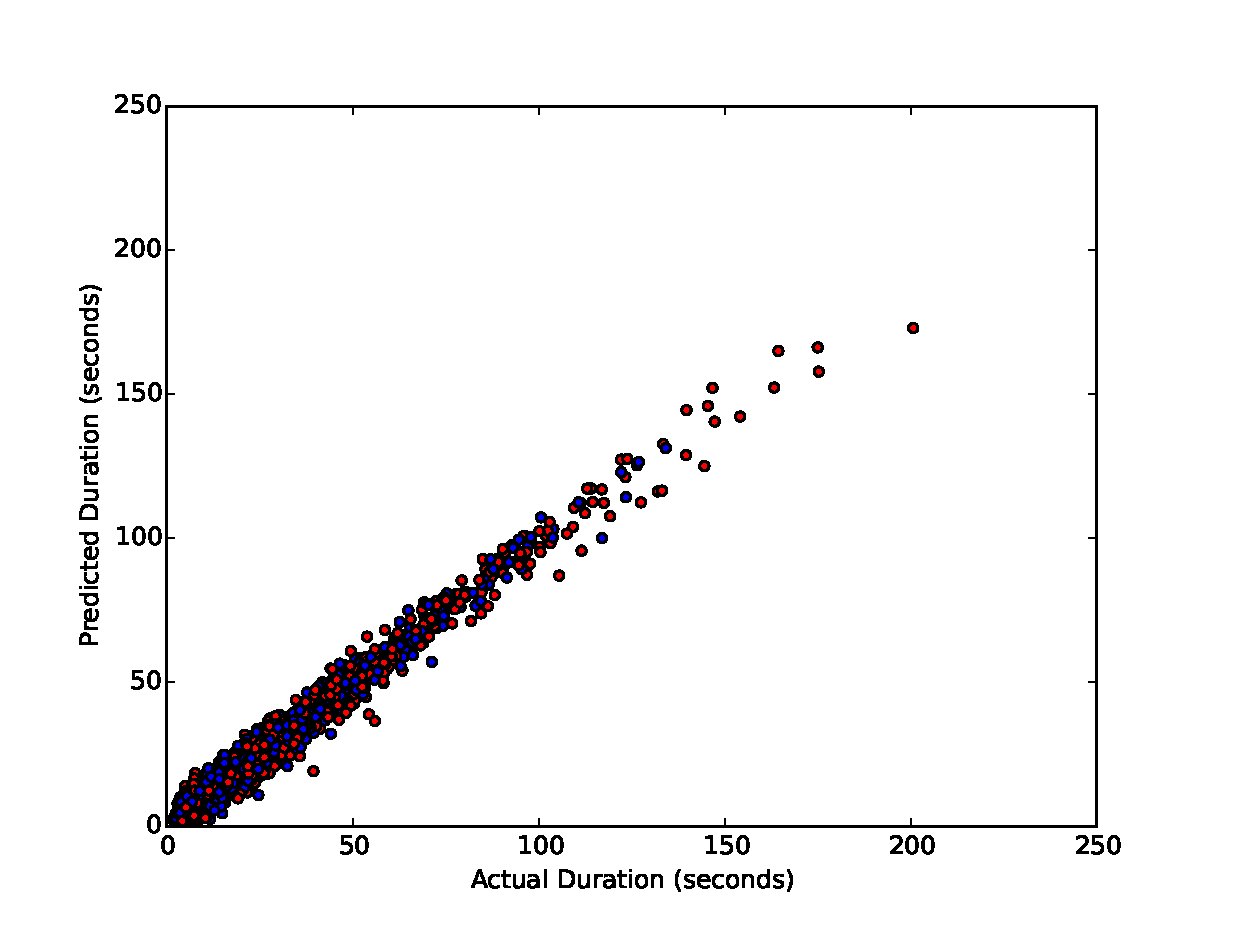
\includegraphics[width=4in]{part11scatter5mer}

$r^2=0.98$

